%%
%% Template intro.tex
%%

\chapter{Background}
\label{cha:back}

\section{Social Networks}
\label{sec:sn}

The social network central for this study is Facebook. Once registering, Facebook users have the option of setting up a personalised profile, they can then establish
 themselves as friends of other users. Friends can interact via wall posts, conversations or by liking some facebook element.

Social networks such as Facebook provide a wide array of user preferences (link, tag, photo, video likes) in an array of interaction mediums and modalities 
(outgoing, incoming) as well as user specific information (gender, age, location, group memberships, favorite movies) and conversation content.

A problem with the Facebook paradigm in relation to this analysis is the requirement for assumed dislikes, if a user does not like some link can we 
imply the user does not like this link? Given the time period Facebook shows a link and the differing online times for Facebook users, this is generally 
a poor assumption. As such a Facebook app named LinkR was developed by NICTA which explicitly stores like and dislike data for users. This app will 
be discussed in the following section.

\section{Data Set}
\label{sec:data}

The LinkR Facebook app was used to collect information about users, their interactions and preferences. The data set contains information about app users as 
well as a sub-set of visible information about their friends. The app tracked and stored information for over 100 app users and their 39,000+ friends.

The four main interactions between users are posts (posting an element on a friends' wall), tags (being mentioned in a friends post or comment), 
 comments (written data on a post) and likes (clicking a like button if a user likes a post or comment). The table below outlines data collected during 
 app trials.

\begin{table}[!htbp]
\centering
	\begin{tabular}{|l|r|r|r|r|} % cols: (left, center, right)
		\hline
		\textbf{App Users} & \textbf{Posts} & \textbf{Tags} & \textbf{Comments} & \textbf{Likes}  \\ \hline
		\textbf{Wall} & 27,955 & 5,256 & 15,121 & 11,033 \\ \hline
		\textbf{Link} & 3,974 & - & 5,757 & 4,279 \\ \hline
		\textbf{Photo} & 4,147 & 22,633 & 8,677 & 5,938 \\ \hline
		\textbf{Video} & 211 & 2,105 & 1,687 & 710 \\ \hline
		 \hline
		\textbf{App Users and Friends} & \textbf{Posts} & \textbf{Tags} & \textbf{Comments} & \textbf{Likes}  \\ \hline
		\textbf{Wall} & 3,384,740 & 912,687 & 2,152,321 & 1,555,225 \\ \hline
		\textbf{Link} & 514,475 & - & 693,930 & 666,631 \\ \hline
		\textbf{Photo} & 1,098,679 & 8,407,822 & 2,978,635 & 1,960,138 \\ \hline
		\textbf{Video} & 56,241 & 858,054 & 463,401 & 308,763 \\ \hline
	\end{tabular}
	\caption{Total app user records}
	\label{tab:revpol}
\end{table}

\clearpage

\section{Notation}
\label{sec:notation}


For our analysis we need to define a feature vector for each item in our data set. The feature vectors are composed of the form 
\( F_i \) for each (user, item) pair where \( i \) is an index into the vector and each \( i \) is composed of the cross product of:
\[ i = \{incoming, outgoing\} \times \{post,photo,video,link\} \times \{comment,tag,like\} \]
The alters of \( i \) can then be defined as all users who have interacted with the current user via some interaction \( i \). The column is 
set to \( 1 \) if any of the alters defined by the current set \( i \) have also liked the item associated with the user, otherwise it is set to \( 0 \).

\begin{figure}[h]
	\begin{center}
		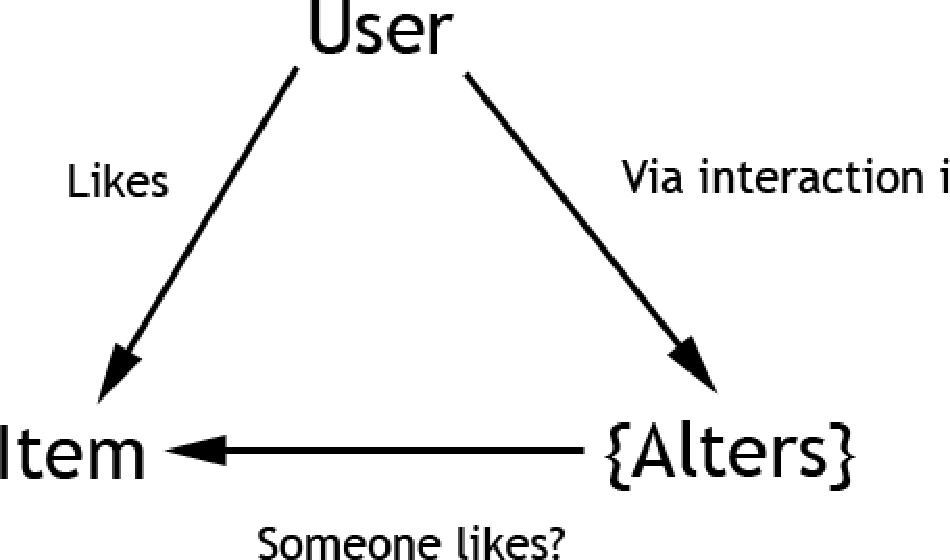
\includegraphics[scale=0.60]{imgs/alters.pdf}
		\caption{Predictors paradigm}
	\end{center}
\end{figure}
\section{Previous Work}
\label{sec:pw}

\subsection{Content Based Filtering}
\label{sec:cbf}

\subsection{Information Diffusion}
\label{sec:id}

\section{Prediction Algorithms}
\label{sec:meth}

\subsection{Constant True}
\label{sec:const}

Refers to the fraction of likes in the current data set which are True.

\subsection{Social Recommender}
\label{sec:sr}

\subsection{Naive Bayes}
\label{sec:nb}

The Naive Bayes classifier is based on applying Bayes' Theorem with independence assumptions. Essentially, the Naive Bayes model assumed that features 
are unrelated to each other given the class variable.

The Naive Bayes model for our model is a conditional model of the form:

\[
 p(C | F_1,\dots,F_n)
\]

Where \( F \) is a feature vector of length \( N \).

Applying Bayes Theorem we obtain:

\[
 p(C|F_1,\dots,F_n) = \frac{p(C)p(F_1,\dots,F_n|C)}{p(F_1,\dots,F_n)}
\]

\subsection{Logistic Regression}
\label{sec:lr}

http://alias-i.com/lingpipe/

\subsection{Support Vector Machine}
\label{sec:svm}

"Support Vector Machines, define a set of basis functions that are centerred on the training data points and then select a subset of these 
during training. Although the training involves nonlinear optimisation, the objective function is convex, and so the solution of the optimisation 
problem is relatively straightforward. The SVM is a decision machine and so does not provide posterior probabilities."

http://www.csie.ntu.edu.tw/~cjlin/liblinear/

\section{Training and Testing}
\label{sec:tt}

All evaluation is done using 10 fold cross validation wherein the data is partitioned into 10 complimentary subsets, each subset is composed of 
two separate parts one section is used for training and the other is used for testing. 
This is performed on 10 distinct subsets and the results are averaged.

An inherent issue in Facebook in terms of this analysis is Facebook's lack of a dislike button, to encourage people to post and interact on Facebook 
users are only given an option to like posts. For the purpose of this analysis we look at two different approaches to over coming this problem. Firstly, 
using the data provided by the linkR app, we have known likes and dislikes data, this will be refered to as our Active data set. Additionally, by using 
"raw" Facebook data we can imply user dislikes by their lack of likes, this will be refered to as our Passive data set.


\section{Evaluation Metrics}
\label{sec:notation}

When evaluating the success of each method at correctly predicting the classification, the following metrics will be used.
A true positive prediction refers to when the classifier correctly identifies the class as true. A false positive occurs when the prediction 
is true, but the true class was false. A false negative occurs when the prediction is false but the actual class is true.



Accuracy relates to the closeness of the true value. In the context of our results, the accuracy refers to the number of correct classifications 
divided by the size of the data set.

\[
 \text{accuracy} = \frac{\text{number of correct classifications}}{\text{size of the test data set}}
\]



Precision relates to the number of retrieved predictions which are relevant. In the context of our results, the precision refers to the number of true positive predictions 
divided by the sum of the true positive and false positive predictions.

\[
 \text{precision} = \frac{\text{number of true positives}}{\text{number of true positives + number of false positives}}
\]

Recall refers to the number of relevant predictions that are retrieved. In the context of our results, recall refers to the number of true positive predictions 
divided by the sum of the true positive and false negative predicitons.

\[
 \text{recall} = \frac{\text{number of true positives}}{\text{number of true positives + number of false negatives}}
\]


The f-score combines and balances both precision and recall and is refered to as the weighted average of both precision and recall. 

\[
 \text{f-score} = 2 \times \frac{\text{precision} \times \text{recall}}{\text{precision} + \text{recall}}
\]

\section{Feature Sets}
\label{sec:features}

%%% Local Variables: 
%%% mode: latex
%%% TeX-master: "thesis"
%%% End: 
